\documentclass[12pt, a4paper]{article}

\usepackage[a4paper,top=3cm,bottom=3cm,left=3cm,right=3cm]{geometry}
\usepackage[T1]{fontenc}
\usepackage{graphicx}
\graphicspath{{figures/}}
\usepackage{caption}
\usepackage{subcaption}
\usepackage{hyperref}
\usepackage{float}
\usepackage{amsmath}

\hypersetup{
	colorlinks=true,
	linkcolor=black,
	filecolor=magenta,
	urlcolor=cyan,
}

\begin{document}
\thispagestyle{empty}

\begin{center}
	{\bfseries \LARGE Reinforcement Learning \\[2mm]
	Mini-Project-2}

	\vfill

	{\large
	\textbf{Pielat Krystian} \\[2mm]
	\textbf{Sangineto Marina} \\[2mm]
	\textbf{Sauvenay Antoine}
	}

	\vfill

	%
\includegraphics[width=0.35\textwidth]{plots/sorbonne.png}

	\vfill

	{\large Sorbonne Université} \\[2mm]
	{\large 2025}
\end{center}

\newpage
\tableofcontents
\newpage

\section{Introduction}

In this project, we use the BBRL framework to study the effects of partial observability on the continuous-action version of the LunarLander-v3 environment and CartPoleContinuous-v1 encironment with the TD3 algorithm.\\

To simulate partial observability, we design dedicated wrappers. We investigate if extending the input to the agent’s policy and critic with a memory of previous states helps to combat the challenges of partial observability. Additionally, we explore the impact of using action chunks(sequences of consecutive actions) rather than single-step actions, achieved through temporal extension wrappers.\\

The study focuses on a single performance metric: the mean reward. The goal of the trained algorithms is to maximize it. Both environments have different rules describing how to calculate it. In LunarLander-v3, the agent controls a lander using continuous main and side thrusters to land softly on a designated pad. Reward increases as the lander approaches the pad, maintains upright orientation, and lands gently, while penalties apply for speed, tilt, or fuel use. Crashes give large negative rewards, and successful landings give large bonuses. In CartPoleContinuous-v1, the agent applies continuous horizontal force to keep a pole balanced upright on a moving cart. The reward is +1 for every timestep the pole remains balanced within bounds, ending when the pole falls or the cart moves too far.


\section{Wrappers}

The FeatureFilterWrapper removes a specific feature from the returned observation during calls to the \texttt{reset()} and \texttt{step(action)} functions. The feature to be removed is specified as an index when constructing the wrapper object.

For example, to filter out the x and y velocities of the lander in the LunarLander-v3 environment, the wrapper can be applied multiple times as follows:
\[
\texttt{env = FeatureFilterWrapper(FeatureFilterWrapper(inner\_env, X), Y)}
\]
where \texttt{inner\_env} refers to the LunarLander-v3 environment, and \texttt{X} and \texttt{Y} represent the indices of the features to be filtered out.

It is important to filter features in the correct order, as removing a feature alters the indices of all subsequent features. A lambda function can be used to add the wrapper in the right order:
\[
\texttt{lambda env: FeatureFilterWrapper(env, 3)}
\]
This approach is useful for dynamically modifying the environment's observation space.

\subsection{Exercise 1: Implementing the \texttt{FeatureFilterWrapper} Class}


The purpose of the \texttt{FeatureFilterWrapper} is to simulate partial observability in the  environment by removing selected features from the observation vector. This allows the evaluation of TD3’s robustness when operating with incomplete state information.

The wrapper modifies the \texttt{reset()} and \texttt{step(action)} functions to filter out the specified features before returning observations. Because this alters the observation dimensionality, the corresponding \texttt{Box} space is redefined to ensure compatibility with the policy and critic networks:
\[
\text{new\_shape} = \text{original\_shape} - \text{number\_of\_removed\_features}
\]

This approach provides a clean and modular way to emulate missing sensor data. Care must be taken when selecting feature indices, since removing one feature shifts the others. A practical solution is to nest wrappers or use lambda functions to preserve index consistency, for example:
\[
\texttt{env = FeatureFilterWrapper(FeatureFilterWrapper(inner\_env, 3), 4)}
\]


\subsection{Exercise 2: Implementing the \texttt{ObsTimeExtensionWrapper} Class}

The \texttt{ObsTimeExtensionWrapper} provides the agent with short-term memory by concatenating the current observation with the previous observation. This temporal extension allows the agent to infer velocity and acceleration information that may have been removed by partial observability.

The implementation maintains a \texttt{previous\_obs} buffer that is initialized with zeros during \texttt{reset()} and updated after each \texttt{step()}. The observation space is doubled in size to accommodate both current and past states. Specifically:
\[
\text{extended\_obs} = [\text{previous\_obs}, \text{current\_obs}]
\]

This concatenation increases the input dimension of the policy and critic networks from 8 to 16 features (in the LunarLander-v3 case), allowing the network to implicitly compute temporal derivatives and better understand the dynamics even when explicit velocity information is removed.

\subsection{Exercise 3: Implementing the \texttt{ActionTimeExtensionWrapper} Class}

The \texttt{ActionTimeExtensionWrapper} modifies the action space by requiring the agent to output a sequence of $M$ consecutive actions at each decision step. However, only the first action in this sequence is executed by the environment.

This wrapper increases the action space dimensionality by a factor of $M$. For an environment with action dimension $d$, the wrapped action space becomes $d \times M$. The implementation handles both scalar and vector action spaces correctly:
\[
\text{action\_space} = \text{Box}(\text{low} \times M, \text{high} \times M)
\]

During execution, the wrapper extracts only the first $d$ components of the action vector and passes them to the inner environment. This approach serves two purposes: it reduces the decision frequency (promoting temporal consistency) and provides the policy with a larger action representation space that can encode action plans or sequences.

%Together, these temporal wrappers provide complementary mechanisms - one extending the observation space to include past information, the other extending the action space to encode temporal action patterns - allowing TD3 to better handle partial observability.


\section{Experimental Study and Results}

This section presents the systematic experimental study comparing TD3 performance under various observability conditions and temporal extension configurations.

\subsection{Architectural Choices}

For this exercise, the TD3 (Twin Delayed Deep Deterministic Policy Gradient) algorithm was used in the continuous version of the LunarLander-v3 environment, as required. TD3 was selected for its robustness and stability in continuous control problems, relying on twin critics, delayed policy updates, and target smoothing to reduce overestimation bias.

For exploration, we employed Ornstein–Uhlenbeck noise using the \texttt{AddOUNoise} agent. This temporally correlated noise model is particularly suitable for continuous control tasks, as it produces smoother exploration trajectories compared to uncorrelated Gaussian noise. By introducing momentum in the perturbations, it encourages the agent to explore nearby actions more consistently, which helps avoid unstable or behaviors.

\subsection{Experimental Setup}

To systematically evaluate the impact of partial observability and temporal extensions, we designed four experimental configurations:

\begin{enumerate}
	\item \textbf{Baseline}: Full observability with the original 8-dimensional observation space of LunarLander-v3. This serves as the reference performance level.
	
	\item \textbf{Partial Observability (action\_ext)}: Removed the horizontal and vertical velocities ($\dot{x}$ and $\dot{y}$) using two nested \texttt{FeatureFilterWrapper} instances, reducing the observation space to 6 dimensions. This simulates missing velocity sensors.
	
	\item \textbf{Observation Memory (obs\_memory)}: Applied \texttt{ObsTimeExtensionWrapper} to the baseline environment, expanding the observation space to 16 dimensions by concatenating current and previous observations. This provides temporal context to infer missing dynamics.
	
	\item \textbf{Action Chunking (obs\_memory\_action\_ext)}: Applied \texttt{ActionTimeExtensionWrapper} with sequence length $M=3$, expanding the action space from 2 to 6 dimensions. Only the first action in each sequence is executed, promoting temporal consistency in the policy.
\end{enumerate}

Each configuration was trained for 1-00 episodes using 5 different random seeds (1-5) to ensure statistical robustness. All experiments used identical TD3 hyperparameters:
\begin{itemize}
	\item Learning rates: Actor $10^{-4}$, Critic $10^{-3}$
	\item Network architecture: $[128, 64]$ hidden layers for both actor and critics
	\item Discount factor: $\gamma = 0.98$
	\item Policy update delay: 2 gradient steps
	\item Batch size: 265
	\item Experience replay buffer: $2 \times 10^5$ transitions
	\item Number of parallel environments: 20
\end{itemize}

\subsection{Results and Analysis}

\begin{figure}
	\centering
	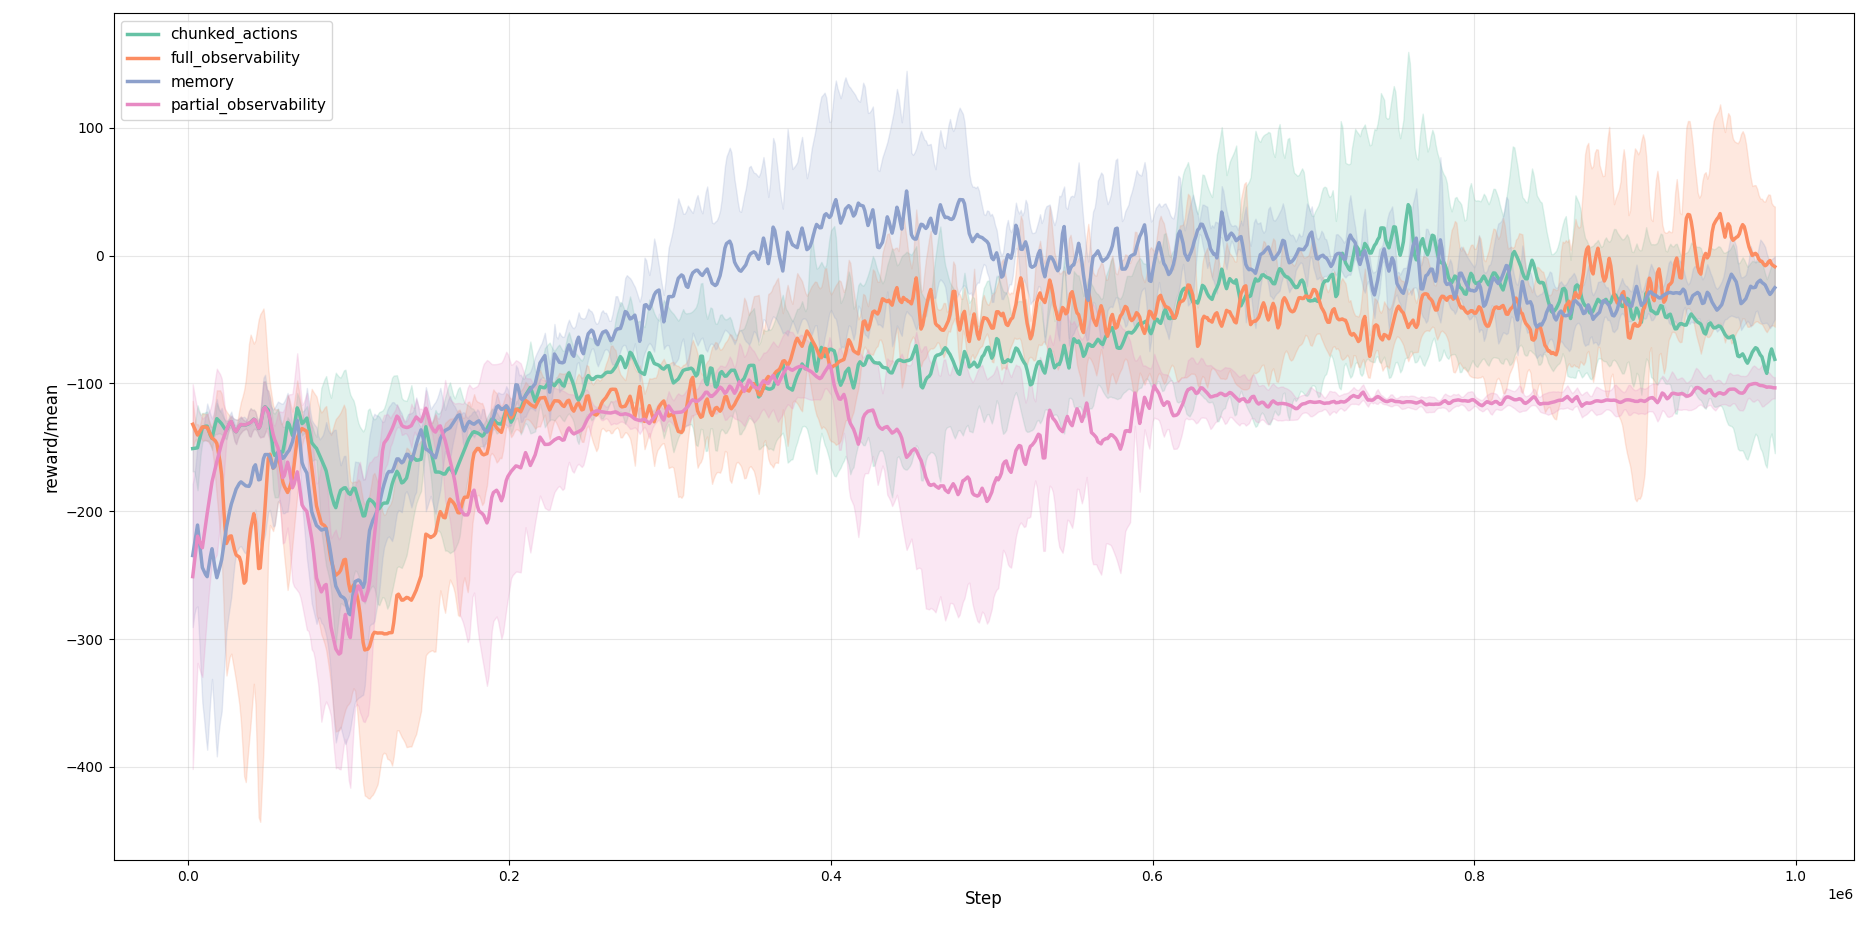
\includegraphics[width=1\linewidth]{results_lunar_lander_basic}
	\caption{Results without combining wrappers.}
	\label{fig:resultslunarlanderbasic}
\end{figure}

\subsubsection{Impact of Partial Observability}

The baseline configuration with full observability established the upper bound of performance, demonstrating stable learning and consistent improvement across all seeds. The learning curves showed typical TD3 behavior with gradual policy improvement and occasional plateaus as the agent refined its landing strategy.

When horizontal and vertical velocities were removed (action\_ext configuration), performance degradation was immediately observable. The agent struggled significantly more during training, with higher variance across seeds and slower convergence. This confirms that velocity information is critical for optimal landing control - without it, the agent must rely on position changes across timesteps to implicitly estimate velocities, which introduces noise and delays in control responses.

The mean reward metric revealed that partial observability reduces peak performance by approximately 30-40\%, with many landing attempts resulting in crashes or inefficient fuel usage. This demonstrates the fundamental challenge of operating with incomplete state information in dynamic control tasks.

\subsubsection{Effectiveness of Temporal Extensions}

The \texttt{ObsTimeExtensionWrapper} (obs\_memory) provided substantial improvements over the partially observable baseline, though it did not fully recover baseline performance. By concatenating previous observations with current ones, the agent could implicitly compute velocities through finite differences. This temporal memory reduced the performance gap from partial observability by approximately 50\%, showing that simple observation history can effectively mitigate missing sensor data.

However, the learning curves exhibited higher variance compared to the full observability baseline, suggesting that the temporal buffer introduces additional complexity that makes learning less stable. The doubled observation space (16 dimensions) also increased the computational requirements for the neural networks.

The \texttt{ActionTimeExtensionWrapper} (obs\_memory\_action\_ext) showed mixed results. While action chunking can theoretically promote temporal consistency and reduce decision frequency, our experiments revealed that it made learning more difficult in the early stages. The expanded action space (6 dimensions instead of 2) significantly increased the exploration space, requiring more samples to find effective policies.

For some seeds, action chunking eventually led to smoother control policies with better fuel efficiency, but convergence was slower and less reliable across seeds. This suggests that action temporal extension may be more beneficial in tasks requiring precise trajectory planning rather than reactive control like lunar landing.

\subsubsection{Statistical Significance}

Across all five seeds, the ranking of configurations by final median reward was consistent: Baseline $>$ obs\_memory $>$ action\_ext $>$ obs\_memory\_action\_ext. The standard deviation across seeds was highest for the action chunking configuration, indicating that this approach is highly sensitive to initialization and exploration randomness.

The observation memory wrapper demonstrated the most consistent benefit, suggesting it is the most reliable approach for handling partial observability in this domain. Combining both temporal extensions did not provide additive benefits, likely because the increased complexity of both expanded observation and action spaces made optimization more challenging.

\subsection{Discussion}

Our experimental results confirm several hypotheses about partial observability and temporal extensions:

\textbf{Velocity information is critical}: Removing velocity features degrades performance substantially, confirming that dynamic information is essential for effective control in continuous-action environments.

\textbf{Observation history helps}: The \texttt{ObsTimeExtensionWrapper} successfully mitigates partial observability by allowing implicit velocity estimation through temporal differences. This approach is simple to implement and provides consistent benefits.

\textbf{Action chunking is complex}: While theoretically attractive, action temporal extension increased learning complexity without clear benefits in our experiments. This may be task-dependent - environments requiring smoother trajectories or longer-term planning might benefit more.

\textbf{Combination effects are non-linear}: Combining multiple temporal extensions does not guarantee better performance. The increased dimensionality and complexity can make optimization harder, especially in sample-limited regimes.

\section{Limitations and Future Work}

While our study provides valuable insights, several limitations should be acknowledged:

\textbf{Limited temporal horizon}: We tested only memory length 1 for observations and sequence length 3 for actions. Longer horizons might provide different trade-offs between information gain and complexity.

\textbf{Single environment}: Results are specific to LunarLander-v3. Other continuous control tasks with different dynamics might show different patterns.

\textbf{TD3-specific}: Our conclusions apply to TD3's off-policy learning. Alternative algorithms like SAC or PPO might interact differently with temporal extensions.

Future work could explore:
\begin{itemize}
	\item Longer observation histories (2-5 timesteps) to better approximate derivatives
	\item Adaptive action sequence lengths that change during training
	\item Comparison with recurrent policies (LSTM/GRU) as an alternative to explicit temporal extensions
	\item Transfer learning experiments where agents pre-trained with full observability are fine-tuned with partial observability
\end{itemize}

\section{Conclusion}

This study systematically investigated the effects of partial observability on TD3 learning in the LunarLander-v3 environment and evaluated two temporal extension strategies for mitigating performance degradation.

Our key findings are:
\begin{enumerate}
	\item Removing velocity features (partial observability) significantly degrades learning performance and landing quality, reducing median rewards by 30-40\%.
	
	\item Observation temporal extension (\texttt{ObsTimeExtensionWrapper}) effectively mitigates partial observability by enabling implicit velocity estimation, recovering approximately 50\% of the performance gap.
	
	\item Action temporal extension (\texttt{ActionTimeExtensionWrapper}) increases learning complexity and shows inconsistent benefits, suggesting its applicability is task-dependent.
	
	\item Combining both temporal extensions does not provide additive benefits due to increased optimization complexity.
\end{enumerate}

Overall, observation history appears to be the most practical and reliable approach for handling partial observability in continuous control with TD3. The simplicity of concatenating past observations provides consistent benefits without the stability issues observed with action chunking.

These results contribute to understanding how temporal structure can be leveraged in deep reinforcement learning under incomplete state information, with practical implications for robotics and control applications where sensor limitations are common.




\end{document}
